\chapter{Physics: Quantum Field Theories}

The Standard Model (SM) of particle physics classifies all known
\index{particle!elementary}
{\it elementary particles}, i.e. particles with no known substructure,
and describes three fundamental forces: the electromagnetic,
weak, and strong forces. Elementary particles can be divided into
\index{particle!matter}
{\it matter particles} (quarks and leptons); {\it gauge bosons}, which mediate
\index{boson!scalar}\index{boson!gauge}
the three aforementioned forces; and a {\it scalar boson}, the Higgs boson,
whose field interacts directly with elementary particles that thereby
acquire their mass. For each particle there exists a corresponding
antiparticle; sometimes a particle is its own antiparticle.
Figure~\ref{fig:SM} gives a schematic overview of the SM.
The SM has a long history of experimental confirmations culminating
in the 2012 discovery of the Higgs boson by the ATLAS and CMS
experiments~\cite{aad_observation_2012,chatrchyan_observation_2012}.
% TODO: maybe it would be fun to include a history here

% brief history according to tong
% e.g. how did QFT start? pauli dirac jordan etc 1920s-30s how to quantize
% fields. Start basically along with discovery of QM. Failing to have 
% theory with infinite num of dof, leading into 2nd world war.
% then tomonaga, schwinger, dyson, feynman. Can renormalize, QED discovered.
% 1970s golden age: asymptotic freedom, infinites understood through
% renormalization group wilson and kadanoff. Progress on understanding geometry
% and topology in QFT.


\begin{figure}
  \centering
  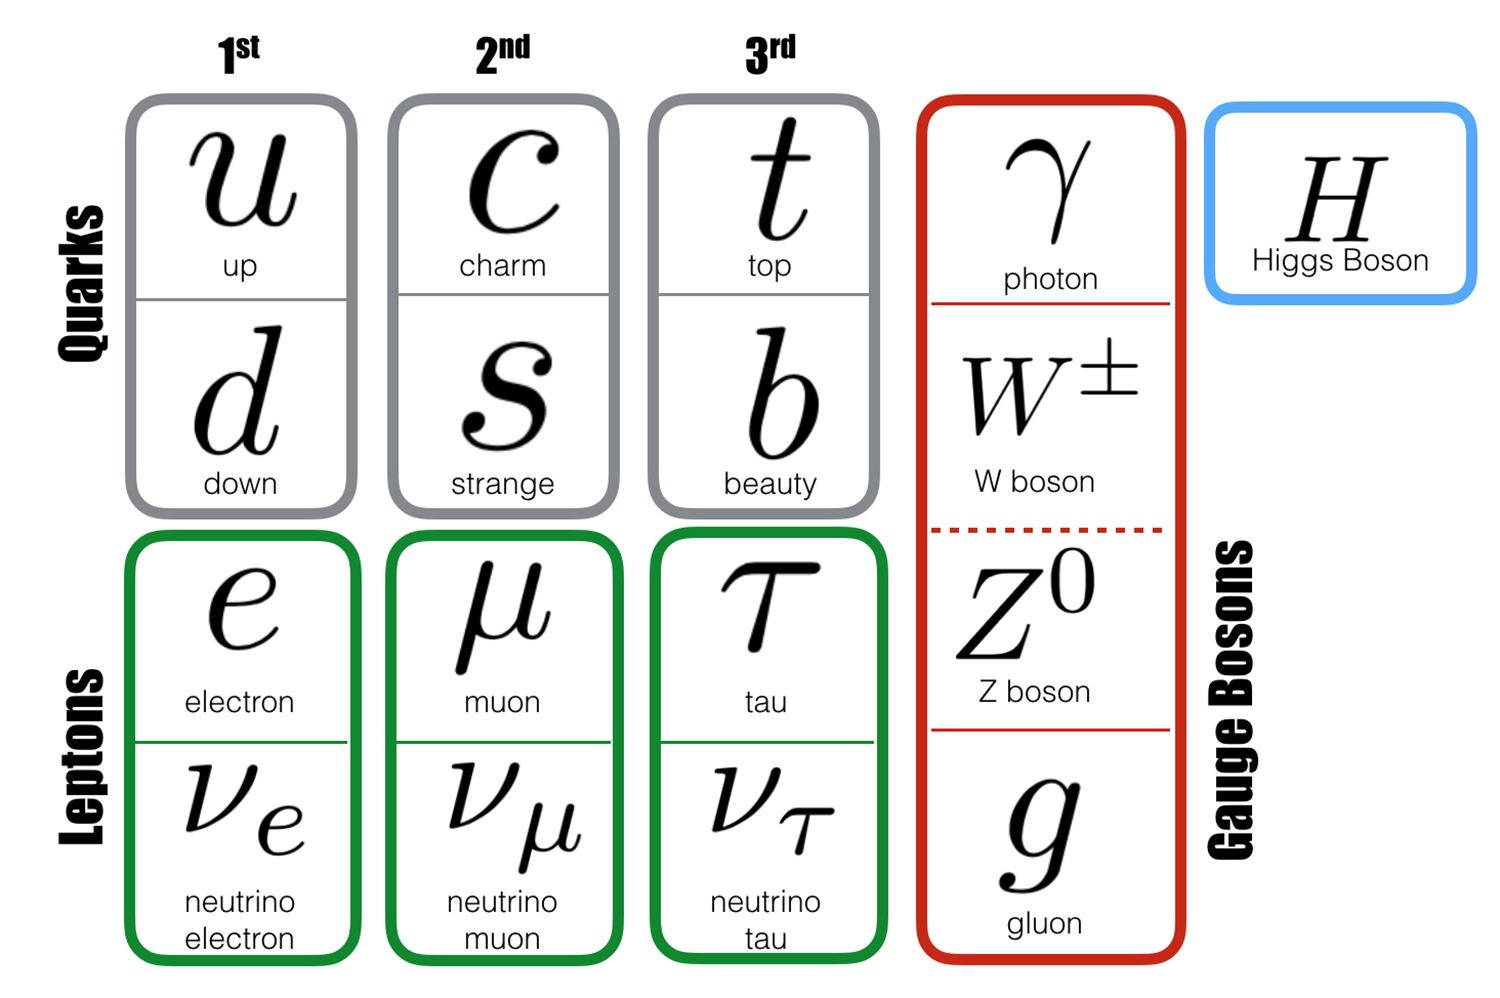
\includegraphics[width=0.80\linewidth]{figs/SM.png}
  \caption{Summary of elementary SM particles. The first three columns give
           the three generations of matter particles. Image taken
           from the Physics Institute at University of 
           Zurich~\cite{zurich_SM}.}
  \label{fig:SM}
\end{figure}

The theoretical framework underlying the SM is an example of a Quantum 
Field Theory (QFT). QFTs are consistent with both quantum mechanics and
relativity. Lattice gauge theories are a kind of QFT; therefore it is
important for the reader to know a little bit about them. There are a lot
of different resources one can use to learn about QFT; for example when I was a
grad student I used Peskin and Schroeder~\cite{peskin_introduction_1995}
and Srednicki~\cite{srednicki_quantum_2007}.
Nowadays there are also some very high quality lectures on YouTube,
for instance a series by Tong~\cite{tongQFT}, which I found had some other nice
introductory remarks.

\section{Introductory remarks about QFT} 

Here I just want to list some things that seem to be true about the universe,
and therefore our underlying theory should reflect these things. For example:
\begin{enumerate}
  \item Causal influences seem to be {\it local}, i.e. there is no
        action-at-a-distance.
  \item Elementary particles are completely and perfectly indistinguishable.
\end{enumerate}
One way to make sense of these two points is to assume the existence of 
{\it fields},\index{field} math objects whose pre-image is all space-time.
That the field value depends on its space-time coordinate allows it to be local,
and all elementary particles are viewed as excitations of the field. Since all
particles are excitations of the same object, it is therefore unsurprising that
they would be indistinguishable.

Related to point (1) above, and as already mentioned in the introduction, we
would like our theories to have this property:
\begin{enumerate}
  \setcounter{enumi}{2}
  \item QFT should be consistent with special relativity.
\end{enumerate}
Demand (3) leads in part to the Klein-Gordon and Dirac equations, and from these
we will find that particle number is not conserved.
A fundamental QFT length scale can be heuristically derived from this statement 
as follows: Consider an elementary particle in a box of length $L$. By the 
uncertainty principle, we have
\begin{equation}
  \Delta p\gtrsim \hbar/2L,
\end{equation}
which means according to relativity,
\begin{equation}
  \Delta E\gtrsim \hbar c/2L.
\end{equation}
If the energy uncertainty is large enough, i.e. large enough to support a
particle-antiparticle pair, we conclude
\begin{equation}
  \Delta E\approx 2mc^2 \gtrsim\hbar c/2L.
\end{equation}
Appearing in this equation is the {\it Compton wavelength}\footnote{I guess if
one uses $\hbar$ instead of $h$ this is rather the {\it reduced} Compton
wavelength. But I somehow always work using $\hbar$ instead of $h$, so I opted
to abuse this convention a little.}\index{wavelength!Compton}
$\lambda_c=\hbar/mc$. This delivers an interpretation for the Compton wavelength:
\begin{equation}
  L \gtrsim \lambda_c/4
\end{equation}
is a distance threshold\footnote{I have also seen $\lambda_c/2$ as the threshold,
which comes when you think the energy uncertainty only has to be large enough to
support a single particle. But in QFT particles are always created from the
vacuum in particle-antiparticle pairs due to conservation laws.} below which 
you have to worry about QFT. Below this scale, you are likely to detect
particle-antiparticle pairs of the species you are examining, which you cannot
distinguish, and it becomes difficult to speak a unique particle at all. In that
sense the Compton wavelength gives a characteristic length scale for a
particle. One can compare this with the particle's de Broglie wavelength
\index{wavelength!de Broglie}$\lambda_v=\hbar/mv$, where it behaves in a well-defined way as a wave.


\section{The principle of stationary action}


This section follows a fairly well known and delightful lecture by Feynman
\cite{caltech}.

\index{classical limit}\index{non-relativistic limit}
\section{The non-relativistic and classical limits}

In this section I briefly give some intuition for how mundane Newtonian
physics can be recovered from the more esoteric relativistic and quantum
theories. Namely I want to focus on the following two phrases:
\begin{enumerate}
  \item The non-relativistic limit is $c\to\infty$.
  \item The classical limit is $\hbar\to0$.
\end{enumerate}
I don't think I have the understanding to prove anything, but at least I
can provide some ideas and examples that can make you believe these
two statements.

The non-relativistic limit is, I think, the easier to understand. When we
learn about relativity, the speed of light $c$ is taken as a ``cosmic speed
limit"; correspondingly, sending $c\to\infty$ lifts the speed limit, and
so perhaps it's not surprising that Galilean physics is recovered.
More explicitly, we can see what happens to the Lorentz factor $\gamma$ and
Einstein velocity addition formula under these limits. For the former
we find
\begin{equation}
  \lim_{c\to\infty}\gamma
  =\lim_{c\to\infty}\frac{1}{\sqrt{1-v^2/c^2}}=1,
\end{equation}
i.e. there is no longer any time dilation or length contraction.
Meanwhile when $c\gg v$, we find for the velocity addition formula 
\begin{equation}
  v_1\oplus v_2
  =\frac{v_1/c + v_2/c}{1+v_1v_2/c^2}
  \approx \frac{v_1}{c} + \frac{v_2}{c}, 
\end{equation}
i.e. it reduces to Galilean velocity addition.

For the classical limit, one can look at specific, simple examples, such as
the quantum harmonic oscillator. In QM, the energy levels of this system
are given by
\begin{equation}
  E_n=\hbar\omega\left(n+\frac{1}{2}\right).
\end{equation}
In the $\hbar\to0$ limit, one therefore sees that the differences in energy
become continuous rather than discrete. More generally one can look at
the Heisenberg uncertainty relation,
\begin{equation}
  \Delta p\Delta x\geq \frac{\hbar}{2},
\end{equation}
and when $\hbar=0$, you are once again allowed to know position and
momentum simultaneously.

\section{The path integral}

\bibliographystyle{unsrtnat}
\bibliography{bibliography}
